\section{Diskussion}
\begin{frame}[t]{Diskussion}
    
    \begin{itemize}\pause
        \item Beschleunigung 
    \end{itemize}
    %Energieerhaltung gut -> Konstanter Verlust durch Reibung 
    %Theorie wohl quatsch, da Reibung und Seilkräfte auch eine große Rolle spielen 
\end{frame}


\begin{frame}{Diskussion Extra}
    \begin{figure}   
    
    \centering
    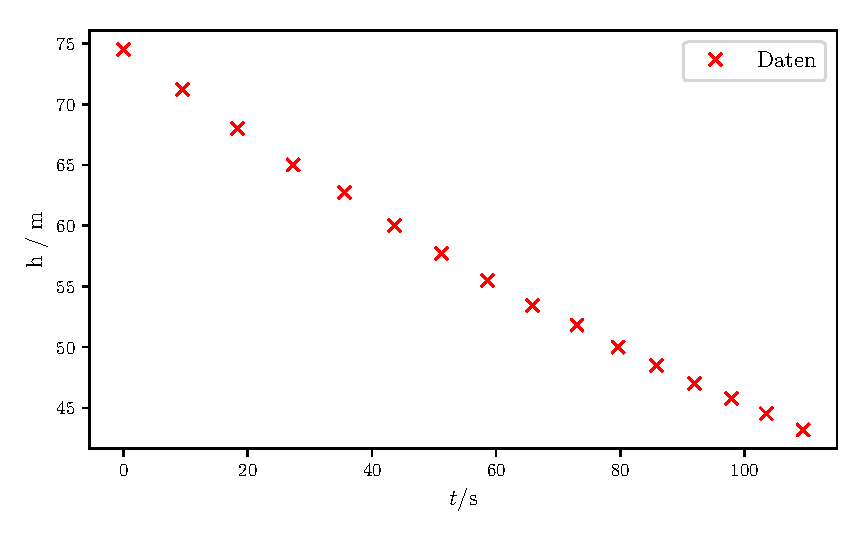
\includegraphics[width=10cm, height=6cm]{plotnew2.pdf}
    \caption{Die Summe der Zeiten gegen die Höhe aufgetragen. Eine e-Funktion könnte zu erkennen sein.} 

    \label{fig:plotnew2}
\end{figure}
\end{frame}


\begin{frame}{Diskussion}
    \begin{figure}   
    
    \centering
    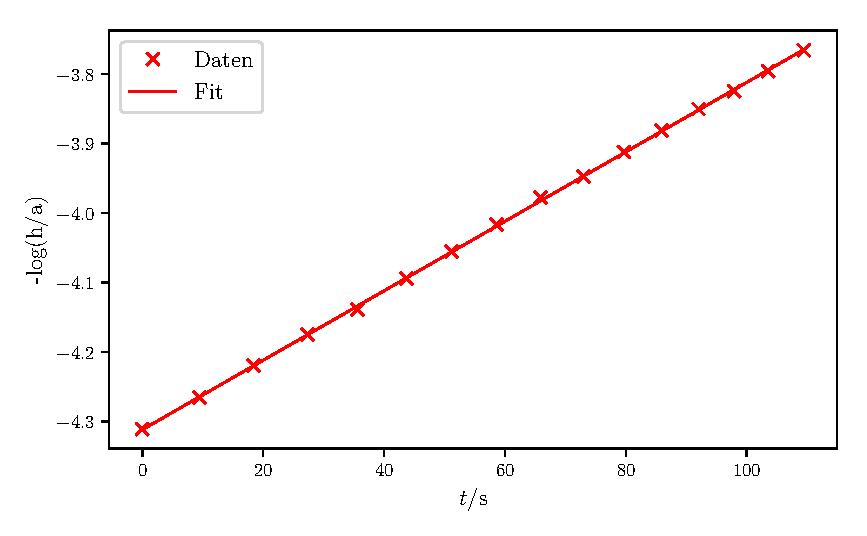
\includegraphics[width=10cm, height=6cm]{plotnew1.pdf}
    \caption{Die Steigung gibt den Dämpfungsfaktor $\lambda$ an. Es ist die Zeit gegen die negative logarithmierte Höhe aufgetragen.} 

    \label{fig:plotnew1}
\end{figure}
\end{frame}


\begin{frame}[t]{Dämpfungsfaktor}
    \begin{block}{Dämpfungsfaktor}
    
        Steigung der Gleichung 
        \begin{equation}
            -ln(h) = \frac{1}{\lambda} t.
        \end{equation}

        Der Faktor ergibt sich zu $\lambda = \SI{200.0(7)}{\per\second}$.
    \end{block}
\end{frame}

\begin{frame}[t]{Diskussion}
    
    \begin{itemize}
        \item Beschleunigung\pause 
        \item Energieerhaltung
    \end{itemize}
    %Energieerhaltung gut -> Konstanter Verlust durch Reibung 
    %Theorie wohl quatsch, da Reibung und Seilkräfte auch eine große Rolle spielen 
\end{frame}
